\section{Casi d'Uso}
\subsection{Introduzione}
In questa sezione sono presentati i casi d'uso che risultano rilevanti per il prodotto Personal Identity Wallet. 
Essi sono stati individuati e definiti attraverso l'analisi del capitolato d'appalto, gli incontri con il proponente e le riunioni interne del team Project Origin.
Ciascun caso d'uso rappresenta un insieme di scenari che hanno lo stesso obiettivo finale per un utente generico del sistema, definito \textbf{\textit{holder}}.
Le norme e le convenzioni adottate per la stesura di ogni caso d'uso sono descritte in dettaglio all'interno del documento Norme di Progetto.
 \subsection{Codice identificativo}
Ciascun caso d'uso viene categorizzato utilizzando la seguente notazione:
\begin{center}\begin{verbatim}
    CU{ID} - {Nome}
\end{verbatim}\end{center}
Ogni caso d’uso è inoltre definito secondo la seguente struttura:
\begin{itemize}
    \item \textbf{ID}: il codice del caso d’uso secondo la convenzione specificata precedentemente;
    \item \textbf{Nome}:  specifica il titolo del caso d’uso;
    \item \textbf{Attori}:  indica gli attori principali (ad esempio l’utente generico) e secondari (ad esempio entità di autenticazione esterne) del caso d’uso;
    \item \textbf{Precondizioni}:  specifica le condizioni che sono identificate come vere prima del verificarsi degli eventi del caso d’uso;
    \item \textbf{Postcondizioni}:  specifica  le  condizioni  che  sono  identificate  come  vere  dopo  il verificarsi degli eventi del caso d’uso;
    \item \textbf{Scenario  principale}:  rappresenta  il  flusso  degli  eventi,  a  volte  attraverso  l'uso di  una  lista  numerata;
    \item \textbf{Scenario alternativo}: rappresenta il flusso alternativo degli eventi, a volte attraversdo l'uso di una lista numerata;
    \item \textbf{Estensioni}: usate per estendere i casi d'uso attraverso un aumento delle funzioanalità di essi;
    \item \textbf{Inclusioni}:  usate per non descrivere più volte lo stesso flusso di eventi, inserendo il comportamento comune in un caso d’uso a parte.
\end{itemize}
Alcuni  casi  d’uso  possono  essere  associati  ad  un Diagramma UML  dei  casi  d'uso riportante lo stesso titolo e codice.
\subsection{Attori}
\begin{itemize}
    \item\textbf{Holder}: l’Holder è, in generale, un’entità (che può essere un individuo, ma non solo), che potrà gestire le proprie credenziali d’accesso e visualizzarle nel proprio portafoglio digitale. L’Holder utlizzerà questa applicazione per poter richiedere e presentare le proprie credenziali d’accesso comunicando con gli altri due attori, cioè l’Issuer e il Verifier;
    \item\textbf{Issuer (sistema).}
    \item\textbf{Issuer (Admin).}
    \item\textbf{Verifier}: il Verifier è l’entità che ha lo scopo di richiedere e verificare le credenziali fornite dall’Holder per permettere l’accesso a determinate aree o servizi che richiedono utenti verificati. Il Verifier verifica le credenziali d’accesso dell’Holder utilizzando un’infrastruttura chiamata Verifiable Data Registry;
    \item\textbf{Wallet.}
\end{itemize}

\subsection{Elenco dei casi d'uso}
\subsubsection{UC1 - Registrazione al Wallet}
\begin{itemize}
\item \textbf{Attore principale:} Holder.
\item \textbf{Attore secondario}: Wallet. 
\item \textbf{Precondizioni:} L’utente (\textit{holder}) fornisce i seguenti dati per effettuare la registrazione:
\begin{itemize}
    \item familyName;
    \item firstName;
    \item email;
    \item password;
    \item conferma password.
\end{itemize}
\item \textbf{Postcondizioni:} L’utente (\textit{holder}) risulta registrato alla piattaforma del Wallet.
\item \textbf{Scenario principale:} L'utente (\textit{holder}) ha eseguito con successo la registrazione.
\item \textbf{Scenario alternativo:} L'utente (\textit{holder}) non è riuscito ad eseguire la registrazione.
\item \textbf{estensione:} UC4-Visualizzazione Errore.
\end{itemize}

\subsubsection{UC2 - Login al Wallet}
\begin{itemize}
\item \textbf{Attore principale:} Holder.
\item \textbf{Attore secondario}: Wallet. 
\item \textbf{Precondizioni:} L'utente (\textit{holder}) che è registrato al sistema deve inserisce le credenziali di accesso ovvero email e password.
\item \textbf{Postcondizioni:} L'utente (\textit{holder}) una volta inserite le credenziali è riuscito a fare l'accesso al Wallet ed è entrato nel sistema.
\item \textbf{Scenario principale:} Login è andato a buon fine e l'utente  (\textit{holder} si trova all'interno del sistema Wallet.
\item \textbf{Scenario alternativo}: Login non riuscito, l'utente (\textit{holder}) ha fornito delle credenziali (email e password) non valide.
\item \textbf{estensione:} UC4-Visualizzazione Errore.
\end{itemize}

\subsubsection{UC3 - Logout dal Wallet}
\begin{itemize}
\item \textbf{Attore principale:} Holder.
\item \textbf{Attore secondario:} Wallet.
\item \textbf{Precondizioni:} L'utente (\textit{holder}) vuole effettuare il logout dalla piattaforma Wallet.
\item \textbf{Postcondizioni:} L' \textit{holder} è uscito dal sistema Wallet e si trova nella schermata di login.
\item \textbf{Scenario principale:} L'utente (\textit{holder}) è riuscito ad eseguire il logout dal Wallet. 
\end{itemize}

\subsubsection{UC4 - Visualizzazione Errore Wallet}
\begin{itemize}
\item \textbf{Attore principale:} Holder.
\item \textbf{Attore secondario:} Wallet.
\item \textbf{Precondizioni:} Il caso d'uso da cui estende si trova in una situazione di errore.
\item \textbf{Postcondizioni:} Viene visualizzato un errore a schermo. 
\item \textbf{Scenario principale:} Viene visualizzato un messaggio d’errore che può riguardare sia il login che la registrazione in base al caso d’uso a cui l’estensione si riferisce.
\end{itemize}

\begin{center}
  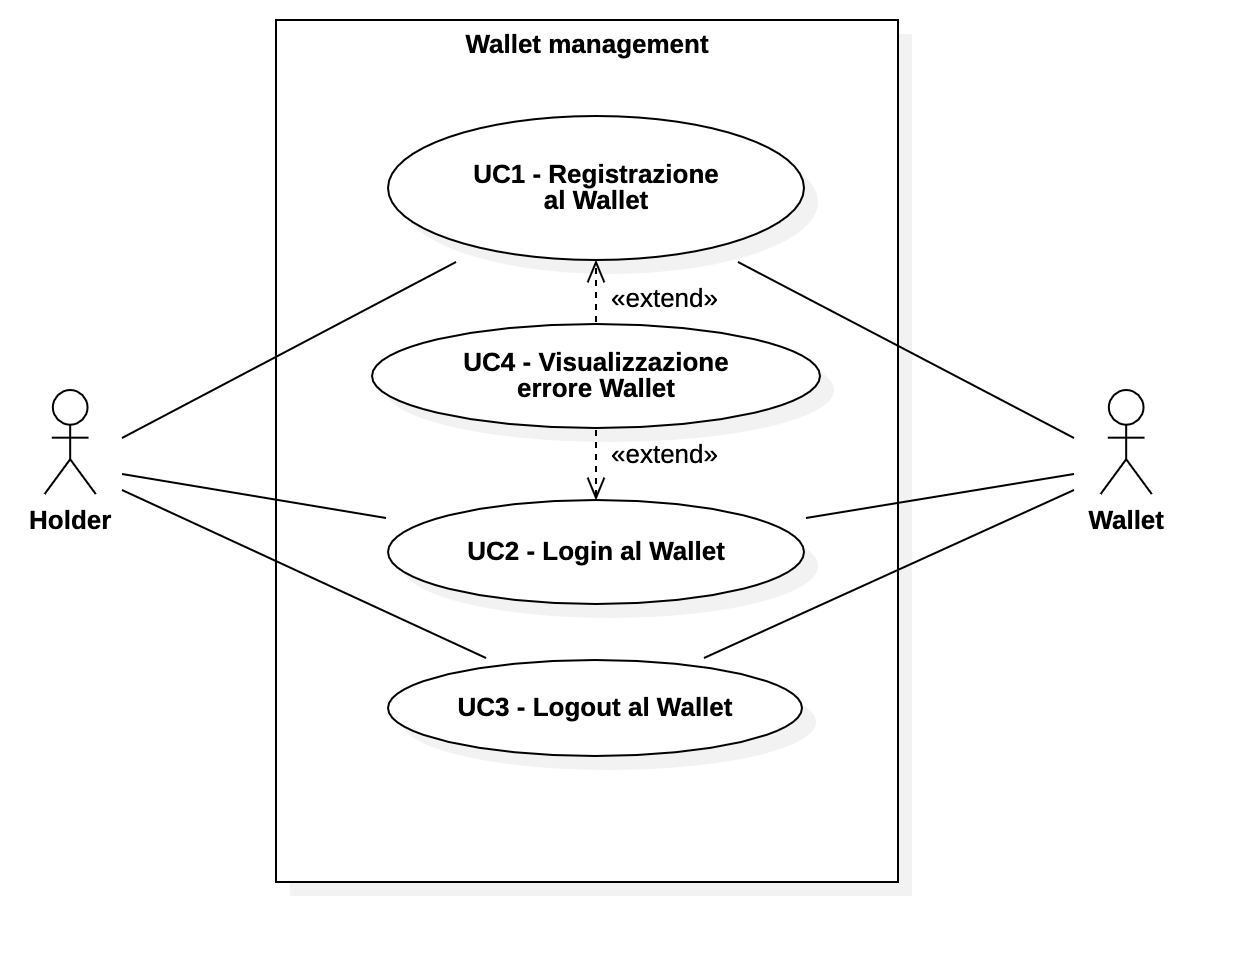
\includegraphics[scale = 0.38]{./res/img/WalletManagement.png}
\end{center}

\subsubsection{UC5 - Registrazione all'Issuer sistema}
\begin{itemize}
\item \textbf{Attore principale:} Holder.
\item \textbf{Attore secondario}: Issuer (sistema). 
\item \textbf{Precondizioni:} L’utente (\textit{holder}) fornisce i seguenti dati per effettuare la registrazione:
\begin{itemize}
    \item familyName;
    \item firstName;
    \item email;
    \item password;
    \item conferma password.
\end{itemize}
\item \textbf{Postcondizioni:} L’utente (\textit{holder}) risulta registrato alla piattaforma dell'Issuer.
\item \textbf{Scenario principale:} L'utente (\textit{holder}) ha eseguito con successo la registrazione alla piattaforma Issuer.
\item \textbf{Scenario alternativo:} L'utente (\textit{holder}) non è riuscito ad eseguire la registrazione.
\item \textbf{estensione:} UC7-Visualizzazione Errore.
\end{itemize}

\subsubsection{UC6 - Login all'Issuer sistema}
\begin{itemize}
\item \textbf{Attore principale:} Holder.
\item \textbf{Attore secondario}: Issuer (sistema). 
\item \textbf{Precondizioni:} L'utente (\textit{holder}) che è registrato al sistema deve inserisce le credenziali di accesso ovvero email e password.
\item \textbf{Postcondizioni:} L'utente (\textit{holder}) una volta inserite le credenziali è riuscito a fare l'accesso al sistema.
\item \textbf{Scenario principale:} Login è andato a buon fine e l'utente  (\textit{holder} si trova all'interno del sistema Issuer.
\item \textbf{Scenario alternativo}: Login non riuscito l'utente (\textit{holder}) ha fornito delle credenziali (email e password) non valide.
\item \textbf{estensione:} UC7-Visualizzazione Errore Issuer.
\end{itemize}

\subsubsection{UC7 - Logout dall'Issuer sistema}
\begin{itemize}
\item \textbf{Attore principale:} Holder.
\item \textbf{Attore secondario:} Issuer (sistema).
\item \textbf{Precondizioni:} L'utente (\textit{holder}), che è già loggato alla piattaforma dell'issuer,  vuole effettuare il logout dalla piattaforma Issuer.
\item \textbf{Postcondizioni:} L' \textit{holder} è uscito dal sistema Issuer e si trova nella schermata di login.
\item \textbf{Scenario principale:} L'utente (\textit{holder}) è riuscito ad eseguire il logout dall'Issuer. 
\end{itemize}

\subsubsection{UC8 - Visualizzazione Errore Issuer}
\begin{itemize}
\item \textbf{Attore principale:} Holder.
\item \textbf{Attore secondario:} Issuer (sistema).
\item \textbf{Precondizioni:} Il caso d'uso da cui estende si trova in una situazione di errore.
\item \textbf{Postcondizioni:} Viene visualizzato un errore a schermo. 
\item \textbf{Scenario principale:} Viene visualizzato un messaggio d’errore che può riguardare sia il login che la registrazione in base al caso d’uso a cui l’estensione si riferisce.
\end{itemize}

\begin{center}
    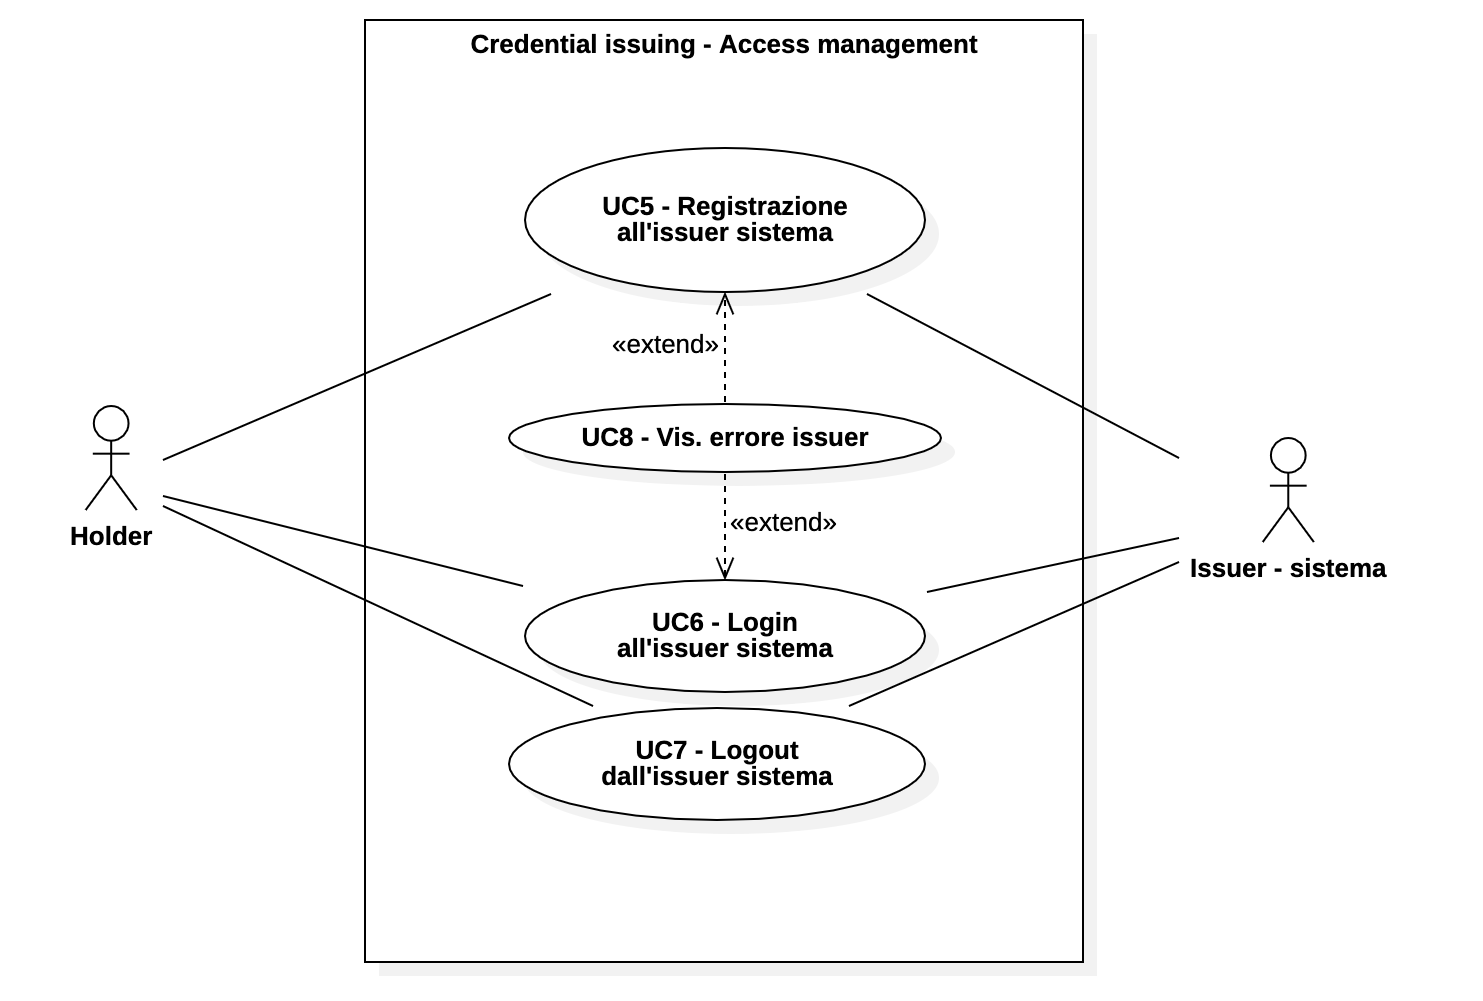
\includegraphics[scale = 0.3]{./res/img/Credential issuing_access.png}
  \end{center}

\subsubsection{UC9 - Richiesta credenziale}
\begin{itemize}
\item \textbf{Attore principale:} Holder.
\item \textbf{Attore secondario:} Issuer (sistema). 
\item \textbf{Precondizioni:} L’ \textit{Holder}, che ha già eseguito il login al sistema di issuer, non è in possesso delle credenziali.
\item \textbf{Postcondizioni:} L’ \textit{Holder} è riuscito a presentare la richiesta per la credenziale nel sito dell'\textit(issuer) ed ora la sua richiesta deve essere esaminata.
\item \textbf{Scenario principale:} 
    \begin{enumerate}
        \item L' \textit{holder} deve richiedere una credenziale; 
        \item l' \textit{holder} naviga nel sito dell \textit{issuer};
        \item l' \textit{holder} presenta una richiesta della credenziale che necessita;
        \item l' \textit{holder} attende che la sua richiesta venga esaminata dall'\textit{Issuer.}
    \end{enumerate}
\item \textbf{Incusioni:}
    \begin{itemize}
    \item UC9.1- Richiesta PID;
    \item UC9.2 - Richiesta EAA;
    \end{itemize}
\end{itemize}

\subsubsection{UC9.1 - Richiesta PID}
\begin{itemize}
\item \textbf{Attore principale:} Holder.
\item \textbf{Attore secondario:} Issuer (sistema). 
\item \textbf{Precondizioni:} L’ \textit{holder} non è in possesso della credenziale identificativa PID, ma ha già eseguito il login nella piattaforma dell'issuer.
\item \textbf{Postcondizioni:} L’ \textit{holder} è riuscito a presentare la richiesta per la credenziale identificativa PID nel sito dell'\textit{Issuer} ed ora la sua richiesta deve essere esaminata.
\item \textbf{Scenario principale:} 
    \begin{enumerate}
        \item L' \textit{holder} deve richiedere una credenziale PID; 
        \item l' \textit{holder} naviga nel sito dell \textit{issuer};
        \item l'\textit{holder} esegue il login nel portale \textit{Issuer sistema};
        \item l' \textit{holder} presenta una richiesta della credenziale PID fornendo i seguenti dati:
        \begin{itemize}
            \item personalId;
            \item dateOfBirth;
            \item familyname;
            \item firstName;
            \item gender;
            \item nameAndfamilyNameAtBirth;
            \item placeOfBirth.
        \end{itemize}
        \item l' \textit{holder} attende che la sua richiesta venga esaminata dall'\textit{Issuer (admin)}
    \end{enumerate}
\end{itemize}

\subsubsection{UC9.2 - Richiesta EAA}
\begin{itemize}
\item \textbf{Attore principale:} Holder.
\item \textbf{Attore secondario:} Issuer (sistema).
\item \textbf{Precondizioni:} L’ \textit{holder} non è in possesso della credenziale EAA, ma ha già eseguito il login nella piattaforma dell'issuer.
\item \textbf{Postcondizioni:} L’ \textit{holder} è riuscito a presentare la richiesta per la credenziale identificativa EAA nel sito dell'\textit(issuer) ed ora la sua richiesta deve essere esaminata.
\item \textbf{Scenario principale:} 
    \begin{enumerate}
        \item L' \textit{holder} deve richiedere una credenziale EAA; 
        \item l' \textit{holder} naviga nel sito dell' \textit{issuer};
        \item l'\textit{holder} esegue il login nel portale \textit{Issuer};
        \item l' \textit{holder} presenta una richiesta della credenziale EAA fornendo i seguenti dati:
        \begin{itemize}
            \item personalId;
            \item familyName;
            \item firstName;
        \end{itemize}
        \item l' \textit{holder} attende che la sua richiesta venga esaminata dall'\textit{Issuer (admin)}
    \end{enumerate}
\end{itemize}

\subsubsection{UC10 - Rilascio credenziale}
\begin{itemize}
    \item \textbf{Attore principale:} Issuer (admin).
    \item \textbf{Attore secondario:} Issuer (sistema).
    \item \textbf{Precondizioni:} L'issuer non ha ancora verificato la richiesta della credenziale del Holder, la richiesta ha come esito 'In Verifica'.
    \item \textbf{Postcondizioni:} L'issuer ha esaminato la richiesta di rilascio della credenziale del Holder, ora la richiesta ha come esito 'Accettata' oppure 'Rifiutata'.
    \item \textbf{Scenario principale:} La richiesta viene esaminata ed ha come esito 'Accettata'.
    \item \textbf{Scenario alternativo:} La richiesta viene esaminata ed ha come esito 'Rifiutata'.
\end{itemize}

\subsubsection{UC11 - Verifica esito richiesta credenziale} 
\begin{itemize}
    \item \textbf{Attore principale:} Holder.
    \item \textbf{Attore secondario:} Issuer (sistema).
    \item \textbf{Precondizioni:} L'Holder, che ha eseguito al login all'interno della piattaforma dell'issuer, non ha verificato l'esito della sua richiesta; lo stato della richiesta gli è sconosciuto.
    \item \textbf{Postcondizioni:} L'Holder ha verificato l'esito della sua richiesta, lo stato della richiesta gli è conosciuto.
    \item \textbf{Scenario principale:} l'\textit{Holder} che ha eseguito il login alla piattaforma dell'issuer può visualizzare lo stato della credenziale richiesta: 
    La sua richiesta può avere 3 stati, 'In Verifica', 'Approvata', 'Rifiutata'.\\
    \item \textbf{Estensioni:}
    \begin{itemize}
    \item  UC13 - Visualizzazione errore rilascio
    \end{itemize}
\end{itemize}

\subsubsection{UC12 - Ottenimento credenziale}
\begin{itemize}
    \item \textbf{Attore principale:} Holder.
    \item \textbf{Attore secondario:} Issuer (sistema), Wallet.
    \item \textbf{Precondizioni:} L'Holder, che ha eseguito al login all'interno della piattaforma dell'issuer, ha verificato l'esito della sua richiesta, la sua richiesta è stata esaminata e ha come esito 'In Verifica', la credenziale non è all'interno del proprio wallet.
    \item \textbf{Postcondizioni:} L'Holder ha la credenziale all'interno del proprio wallet.
    \item \textbf{Scenario principale:} La richiesta della credenziale ha come esito 'Approvata',
    L’Holder aggiunge la credenziale sul proprio wallet accetandola.\\
    La credenziale richiesta è aggiunta al wallet.
    \item \textbf{Scenario alternativo:} La richiesta della credenziale ha come esito 'Rifiutata', l'Holder non può aggiungerla al proprio wallet e la richiesta deve essere rifatta.
\end{itemize}

\subsubsection{UC13 - Visualizzazione errore di rilascio}
\begin{itemize}
    \item \textbf{Attore principale:} Holder.
    \item  \textbf{Attore secondario:} Issuer (sistema).
    \item \textbf{Precondizioni:} Il caso d'uso da cui estende si trova in una situazione di errore.
    \item \textbf{Postcondizioni:} Viene visualizzato un errore a schermo. 
    \item \textbf{Scenario principale:} Viene visualizzato un messaggio d’errore che riguarda il rilascio di una credenziale.
\end{itemize}

\begin{center}
    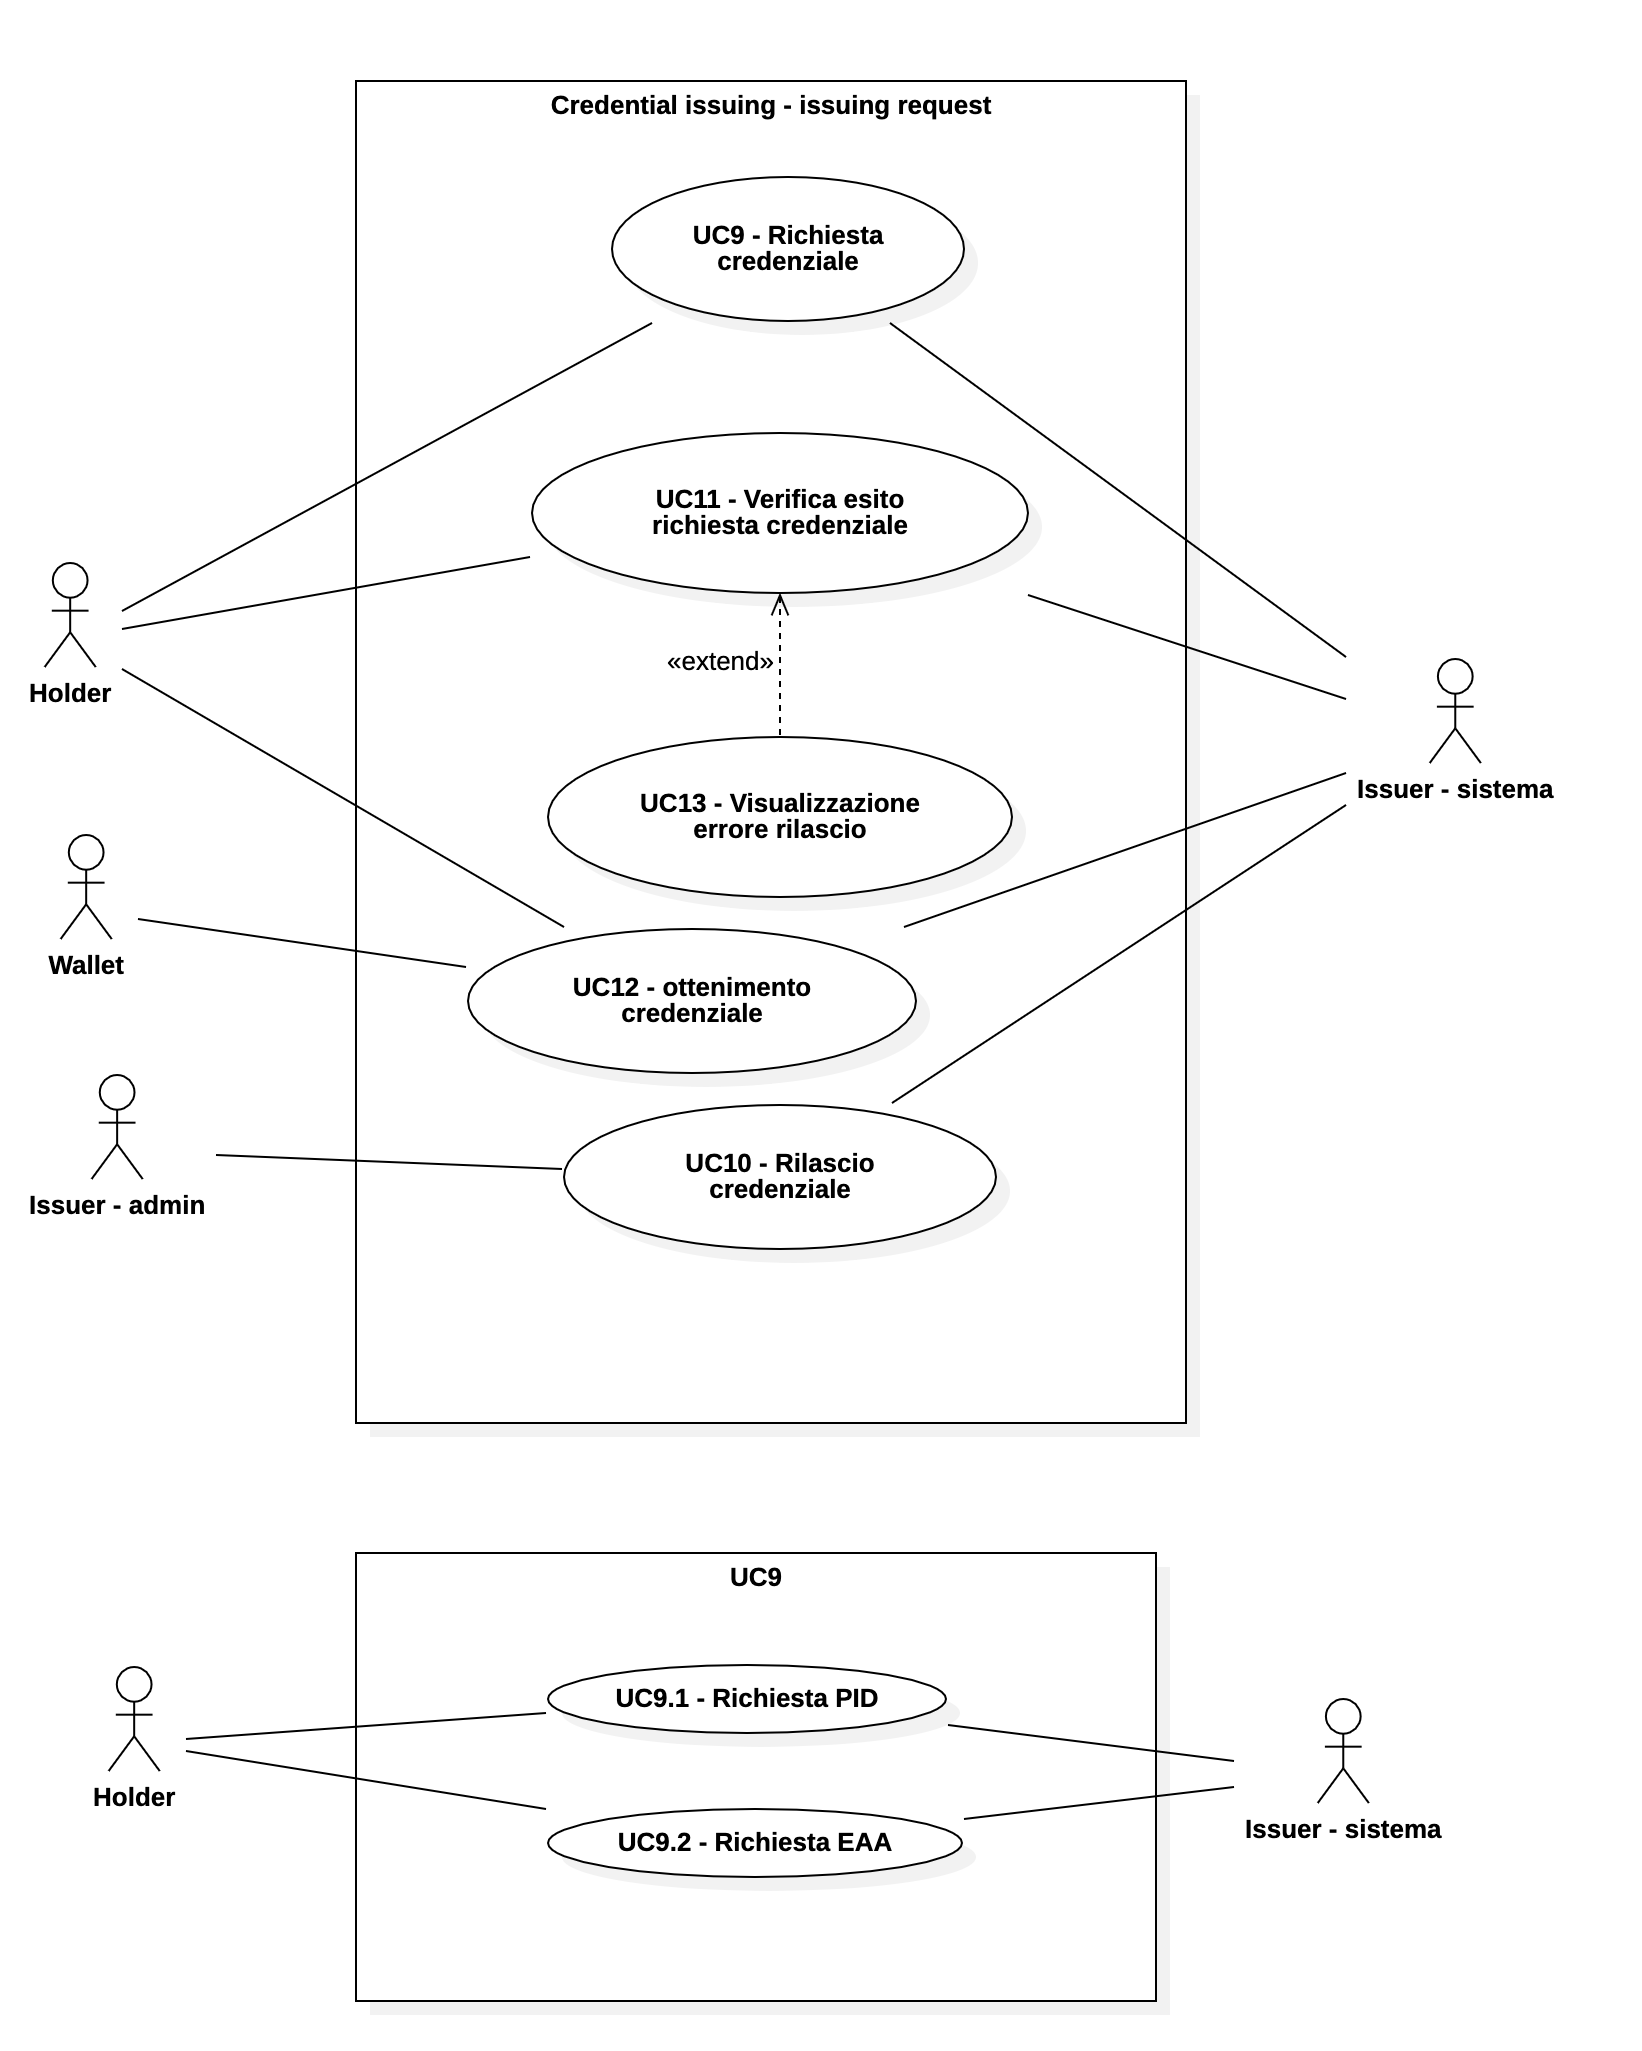
\includegraphics[scale = 0.3]{./res/img/Credential issuing_request.png}
\end{center}

\subsubsection{UC14 - Visualizzazione credenziali}
\begin{itemize}
    \item \textbf{Attore principale:} Holder.
    \item \textbf{Attore secondario:} Wallet.
    \item \textbf{Precondizioni:} l'\textit{holder}, dopo aver effettuato il login al Wallet, vuole visualizzare le credenziali presenti nel Wallet. 
    \item \textbf{Postcondizioni:} l'\textit{holder} riesce a visualizzare correttamente tutta la lista delle credenziali presenti nel suo wallet. 
    \item \textbf{Scenario principale:} Viene visualizzata una lista con tutte le credenziali presenti all'interno del Wallet personale. 
\end{itemize}


\subsubsection{UC15 - Visualizzazione singola credenziale}
\begin{itemize}
\item \textbf{Attore principale:} Holder.
\item \textbf{Attore secondario:} Wallet. 
\item \textbf{Precondizioni:} L’ \textit{holder}, dopo aver effettuato il login al Wallet, vuole visualizzare una credenziale dalla lista delle credenziali contenute all'interno del proprio wallet personale. 
\item \textbf{Postcondizioni:} L’ \textit{holder} è riuscito a visualizzare la singola credenziale di interesse presente nel wallet personale.
\item \textbf{Scenario principale:} 
\item \textbf{Incusioni:}
    \begin{itemize}
    \item UC15.1- Visualizzazione PID;
    \item UC15.2 - Visualizzazione EAA;
    \end{itemize}
\end{itemize}

\subsubsection{UC15.1 - visualizzazione PID}
\begin{itemize}
\item \textbf{Attore principale:} Holder.
\item \textbf{Attore secondario:} Wallet. 
\item \textbf{Precondizioni:} L’ \textit{holder}, dopo aver effettuato il login al Wallet, vuole visualizzare la credenziale identificativa PID.
\item \textbf{Postcondizioni:} L’ \textit{holder} visualizza correttamente la credenziale identificativa PID presente nel proprio wallet.
\item \textbf{Scenario principale:} 
    \begin{enumerate}
        \item L' \textit{holder} vuole visualizzare credenziale PID; 
        \item naviga nella lista delle credenziali presente nel proprio Wallet;
        \item una volta scelta la credenziale Pid da visualizzare può consultarla singolarmente in particolare i seguenti campi:
        \begin{itemize}
            \item id;
            \item issuer;
            \item issuanceDate (data di richiesta);
            \item issued (data di rilascio);
            \item validFrom (data di validità);
            \item personalId;
            \item dateOfBirth;
            \item familyname;
            \item firstName;
            \item gender;
            \item nameAndfamilyNameAtBirth;
            \item placeOfBirth.
        \end{itemize}
    \end{enumerate}
\end{itemize}

\subsubsection{UC15.2 - Visualizzazione EAA}
\begin{itemize}
\item \textbf{Attore principale:} Holder.
\item \textbf{Attore secondario:} Wallet.
\item \textbf{Precondizioni:} L’ \textit{holder}, dopo aver effettuato il login al Wallet,  vuole visualizzare la credenziale EAA.
\item \textbf{Postcondizioni:} L’ \textit{holder} riesce a visualizzare correttamente la credenziale EAA presente all'interno del proprio wallet.
\item \textbf{Scenario principale:} 
    \begin{enumerate}
        \item L' \textit{holder} vuole visualizzare credenziale EAA; 
        \item naviga nella lista delle credenziali presente nel proprio Wallet;
        \item una volta scelta la credenziale Pid da visualizzare può consultarla singolarmente in particolare i seguenti campi:
        \begin{itemize}
            \item id;
            \item issuer;
            \item type;
            \item issuanceDate (data di richiesta);
            \item issued (data di rilascio);
            \item validFrom (data di validità);
            \item exipirationDate (data di scadenza);
            \item status (può essere valido, scaduto, revocato, sospesa);
            \item personalId;
            \item familyName;
            \item firstName;
            \item Attributi attestati;
        \end{itemize}
    \end{enumerate}
\end{itemize}


\subsubsection{UC16 - Cancellazione credenziale}
\begin{itemize}
\item \textbf{Attore principale:} Holder.
\item \textbf{Attore secondario:} Wallet.
\item \textbf{Precondizioni:} L' \textit{holder}, dopo aver effettuato il login al Wallet, vuole rimuovere una credenziale dal suo \textit{Wallet}.
\item \textbf{Postcondizioni:} L' \textit{holder} ha cancellato la credenziale dal suo \textit{Wallet}.
\item \textbf{Scenario principale:} 
    \begin{enumerate}
    \item L'\textit{holder} si trova sulla schermata di una crenziale che vuole cancellare; 
    \item clicca sul pulsante "elimina"; 
    \item clicca sul pulsante "conferma"; 
    \item la credenziale è stata cancellata permanentemente.
    \end{enumerate}
\end{itemize}

\begin{center}
    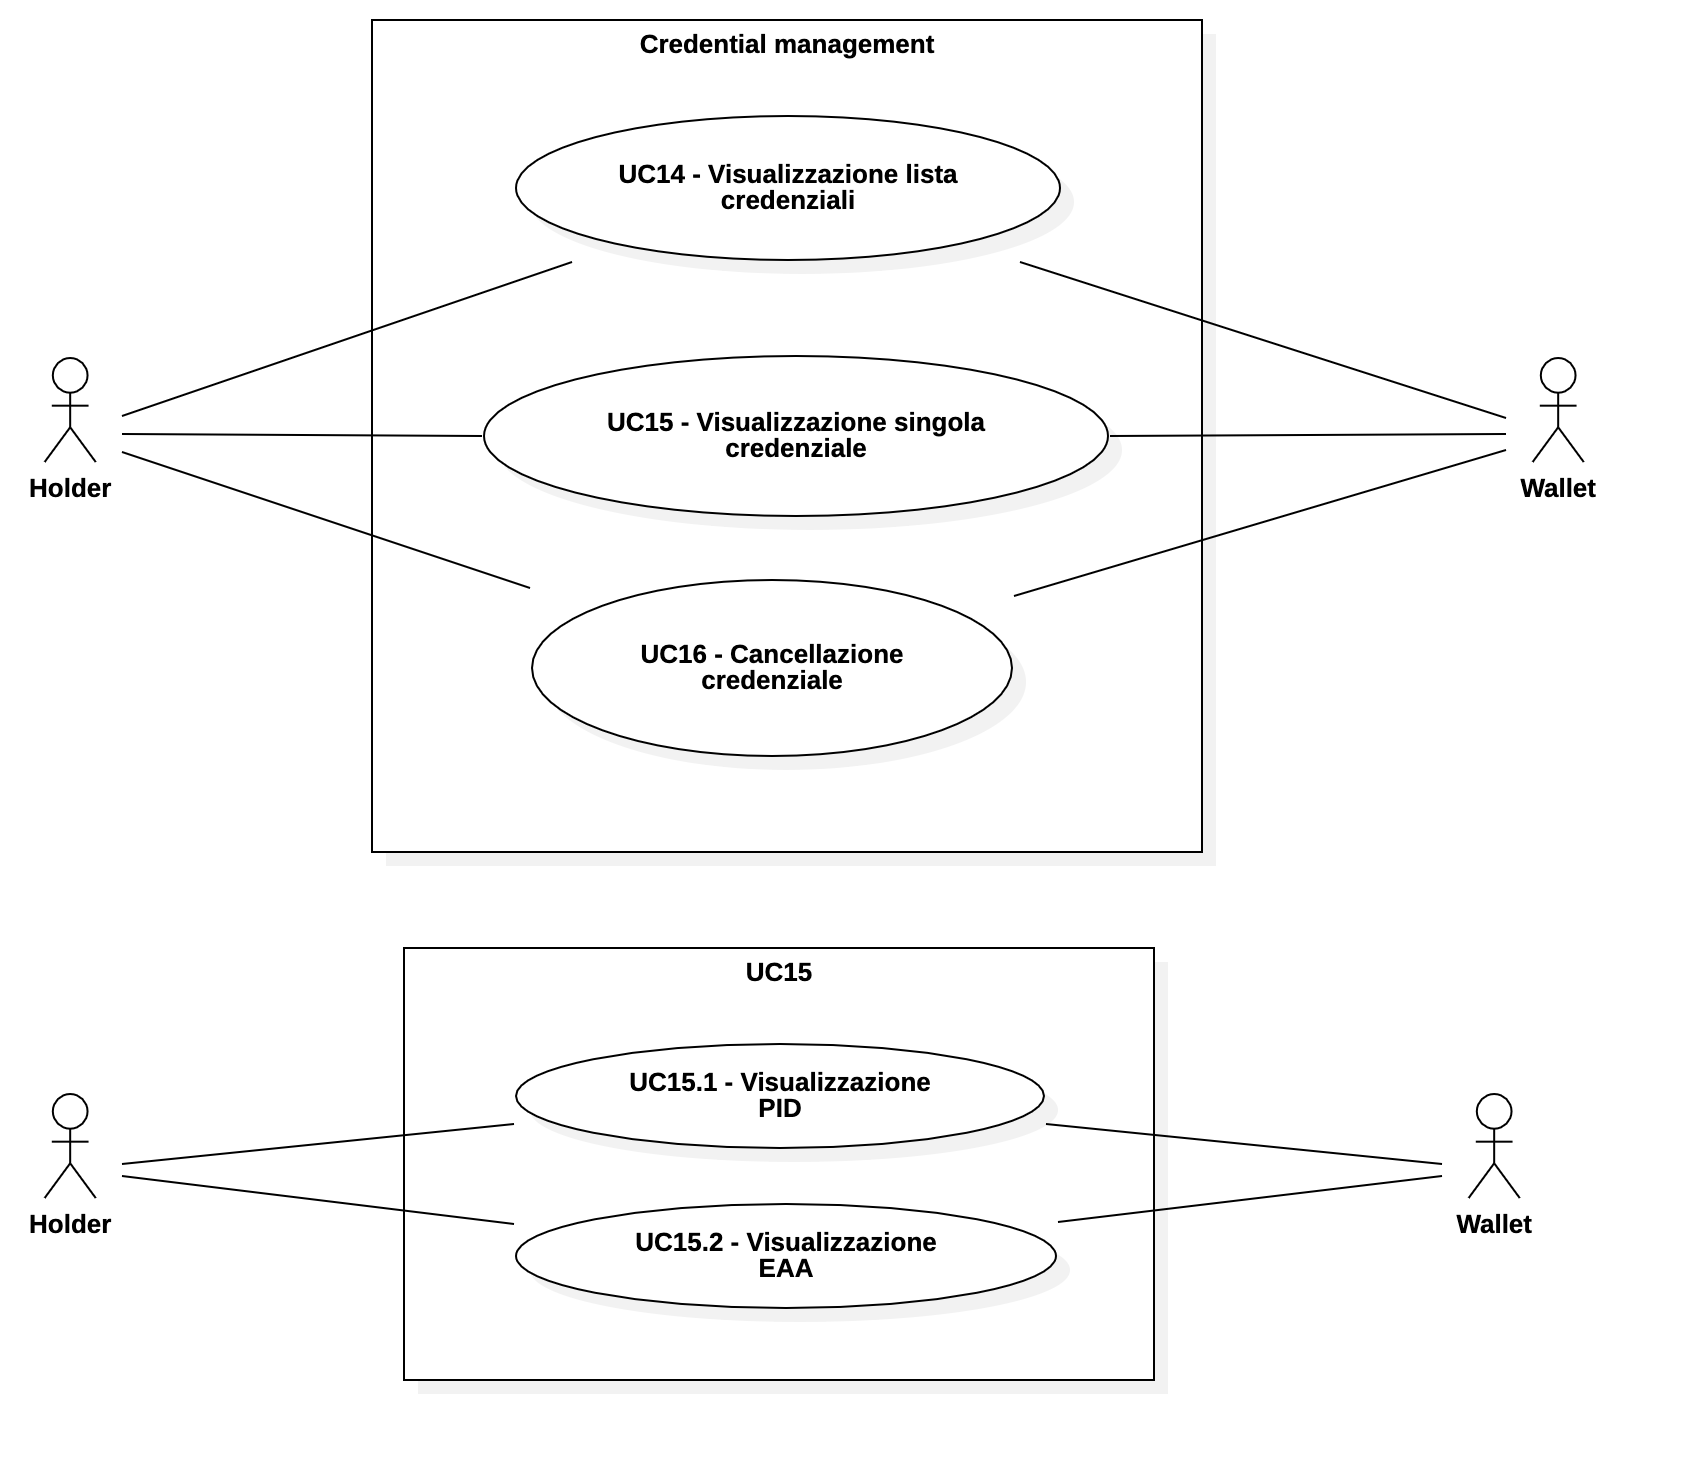
\includegraphics[scale = 0.3]{./res/img/CredentialManagement.png}
  \end{center}

\subsubsection{UC17 - Richiesta credenziali per verifica}
\begin{itemize}
\item \textbf{Attore principale:} Verifier.
\item \textbf{Attore secondario:} Holder.
\item \textbf{Precondizioni:} Il \textit{verifier} deve richiedere una credenziale all' \textit{holder}.
\item \textbf{Postcondizioni:} Il \textit{verifier} ha presentato una richiesta di una credenziale all' \textit{holder}.
\item \textbf{Scenario principale:} 
    \begin{enumerate}
        \item Il \textit{verifier} fa richiesta ad un \textit{holder} di fornirgli una credenziale salvata nel suo Wallet.
    \end{enumerate}
\end{itemize}

\subsubsection{UC18 - Fornitura delle credenziali per verifica}
\begin{itemize}
\item \textbf{Attore principale:} Holder. 
\item \textbf{Attore secondario:} Verifier.
\item \textbf{Precondizioni:} L’ \textit{holder} vuole fornire la credenziale presente nel Wallet personale al \textit{verifier}.
\item \textbf{Postcondizioni:} La credenziale dell’ \textit{holder} è stata fornita al \textit{verifier}.
\item \textbf{Scenario principale:} L' \textit{holder} fornisce con successo la credenziale che gli è stata richiesta dal \textit{verifier}.
\item \textbf{Scenario alternativo:} L' \textit{holder} fornisce delle credenziali non valide e richiama un caso di errore.
\item \textbf{Estensione:} UC15 - Visualizzazione errore di verifica.
\end{itemize}

\subsubsection{UC19 - Visualizzazione errore di verifica}
\begin{itemize}
    \item \textbf{Attore principale:} Holder.
    \item \textbf{Attore secondario:} Verifier.
    \item \textbf{Precondizioni:} Il caso d'uso da cui estende si trova in una situazione di errore.
    \item \textbf{Postcondizioni:} Viene visualizzato un errore a schermo. 
    \item \textbf{Scenario principale:} Viene visualizzato un messaggio d’errore che riguarda la fornitura di una credenziale per la verifica.
\end{itemize}

\begin{center}
    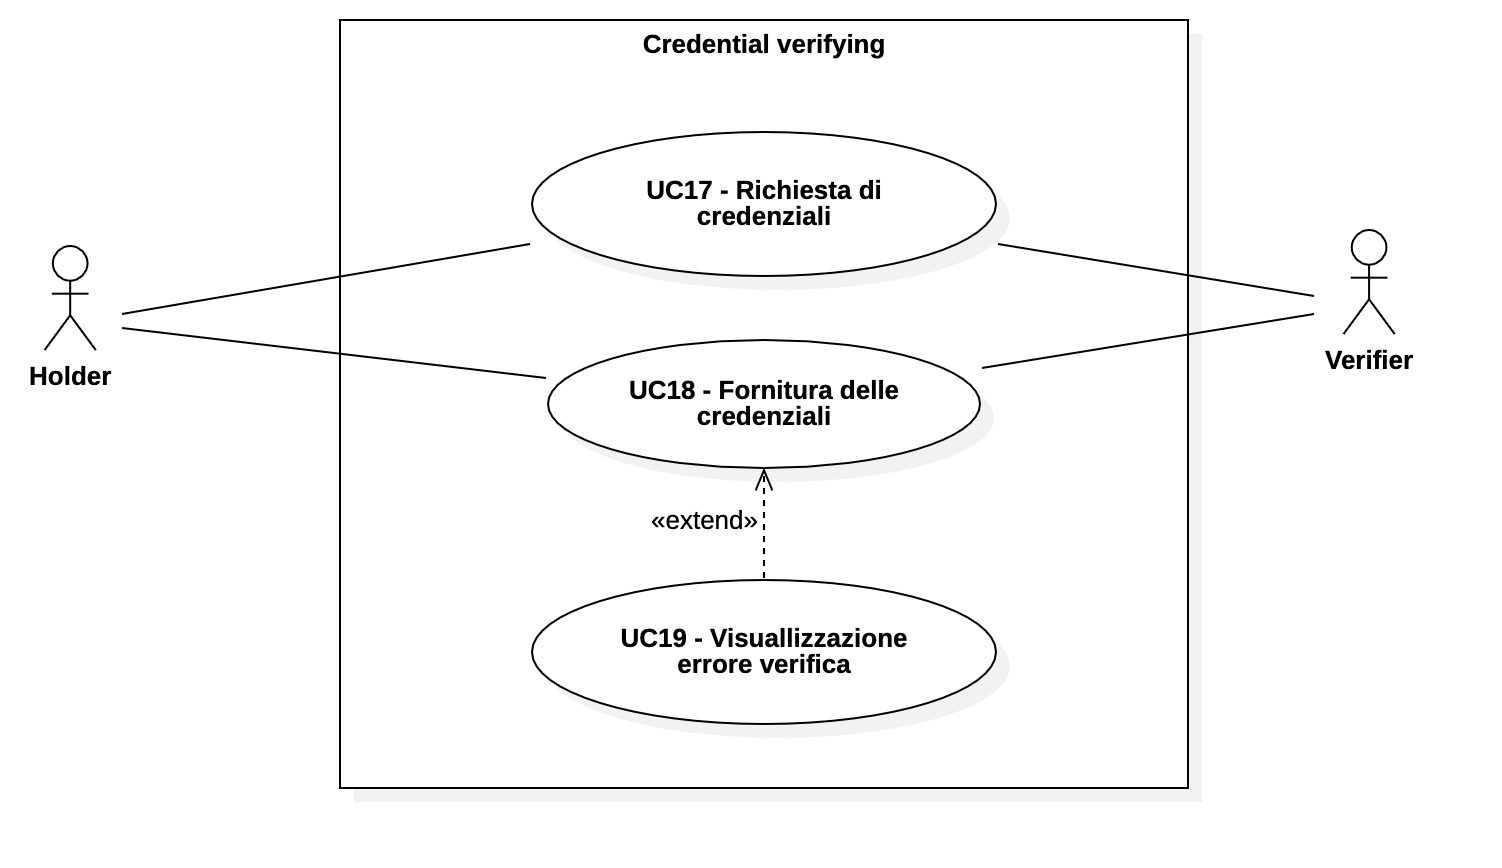
\includegraphics[scale = 0.32]{./res/img/CredentialVerifying.png}
  \end{center}